\documentclass[11pt]{article}
\usepackage[margin=1in]{geometry}
\usepackage[T1]{fontenc}
\usepackage{lmodern}
\usepackage{graphicx}
\usepackage{booktabs}
\usepackage{amsmath}
\usepackage{xcolor}
\usepackage[hidelinks]{hyperref}
\usepackage{enumitem}
\setlist{nosep,leftmargin=1.4em}

\title{Verified Programs Beat Raw Throughput:\\
A Tool-Using Qwen3.8-Flash-Next Agent for ARC-AGI-2 on Four L4 GPUs}
\author{Md.\ Hamid Hosen \and FOYSAL \and Esfer Sami\\[2pt]
\small Team Hack2Publish, ARC Prize 2026}
\date{November 2026}

\begin{document}
\maketitle

\begin{abstract}
We document our ARC-AGI-2 submission 57851995, which scored 54.17\,\% on the public leaderboard, and the measurements behind it.
The system serves Qwen3.8-Flash-Next fully offline on Kaggle's 4$\times$L4 machine with 4-bit (W4A16) routed experts, an FP8 per-layer-embedding table, an FP8 KV cache and 3-token multi-token-prediction (MTP) speculation.
Nine agent sessions run at once; each writes a \texttt{transform(grid)} program in a stateful Python sandbox, scores it on every training pair, and submits the program's output.
Over seven months our other method families stayed lower: reproductions of the NVARC 2025 test-time-training pipeline reached 32.64, a 27B dense model reached 34.58 with direct reasoning and 22.92 as a tool agent, and a faster 3-bit build of the same Flash-Next agent reached 49.58.
Three findings explain the ranking.
(1)~With a strong enough model, the training pairs are a precise free verifier: 25 of 26 submitted train-passing W4A16 attempts were correct.
(2)~Lower precision showed up as false verification rather than as fewer solves: the 3-bit build passed the train check more often per hour, but 13 of its 54 train-passing answers were wrong.
(3)~Memory, not compute, limits L4 serving: FP8 KV fitted 9 sessions where BF16 fitted 5, with no measured loss (13/15 tasks each).
We also report that public evaluation scores rank systems poorly against the leaderboard, and we give the limits of our evidence.
A companion paper analyses where our NVARC-based pipeline lost its score \cite{paper1}.
\end{abstract}

\section{Introduction}
ARC-AGI-2 \cite{arcagi2,arctr2025} asks a solver to produce the exact output grid of an unseen task from a few demonstration pairs, with two attempts per test input. The Kaggle competition runs a notebook on 240 hidden tasks within 12 hours on four 24\,GB NVIDIA L4 GPUs, without internet access.
Reasoning language models solve many ARC tasks when they can think long enough; our 27B runs needed about 60k thinking tokens per attempt to reach their best leaderboard score (Section~\ref{sec:journey}).
On four L4s this turns ARC-AGI-2 into a budget problem:
\begin{equation}
\text{score} \;\approx\; \underbrace{P(\text{task reached in time})}_{\text{coverage}} \times \underbrace{P(\text{solved}\mid\text{reached})}_{\text{solve rate}} .
\end{equation}
Coverage depends on tokens per second and tokens per task; the solve rate depends on the model and on how answers are selected.
This paper shows how our final system raised both, and which changes did not help.

\paragraph{Contributions.}
\begin{itemize}
\item A complete offline recipe for a 512-expert MoE reasoning model on 4$\times$L4 (W4A16 experts, FP8 embedding table and KV cache, MTP speculation, nine concurrent 104k-token sessions), with run-safety rules that always produce a valid submission.
\item A verifying tool agent whose answers are outputs of programs checked on all training pairs, and measurements of how precise that check is at two weight precisions.
\item A record of seven months of leaderboard results across four method families (Figure~\ref{fig:lb}), including the negative ones.
\end{itemize}

\section{Background and prior work}
\paragraph{Test-time training (TTT).} The ARChitects \cite{architects2024} and NVARC \cite{nvarc2025} fine-tune a small grid model on each task at test time and rank sampled candidates with augmentation-based scores. TRM \cite{trm} trains a tiny recursive network. Our companion paper \cite{paper1} decomposes the score of our NVARC-derived notebooks into generation and selection and finds that, under the shared settings, most lost test inputs never received a correct candidate.
\paragraph{Reasoning and refinement.} Long-thinking LLMs answer directly or refine their answer over iterations, as in Poetiq's solver \cite{poetiq}. Program induction with LLMs writes code and checks it on the demonstrations \cite{greenblatt2024}.
\paragraph{Agents.} Our solver started from the ``Duck'' tool-agent harness used for ARC-AGI-3 \cite{duck}, which gives a model a persistent Python tool. We adapted it to static ARC-AGI-2 grids and added a training-pair checker and an explicit \texttt{submit} call.
\paragraph{Serving.} We use a vLLM-0.32-based engine (Merlin 3.0.0) \cite{vllm} with Marlin-style 4-bit MoE kernels and MTP speculation \cite{qwen38}.

The new element is the combination: a large sparse model at low precision on small GPUs, with a program-level verifier inside every attempt instead of voting over sampled grids.

\section{The path to the submission}\label{sec:journey}
Figure~\ref{fig:lb} shows every scored submission of our team.
\begin{figure}[t]
\centering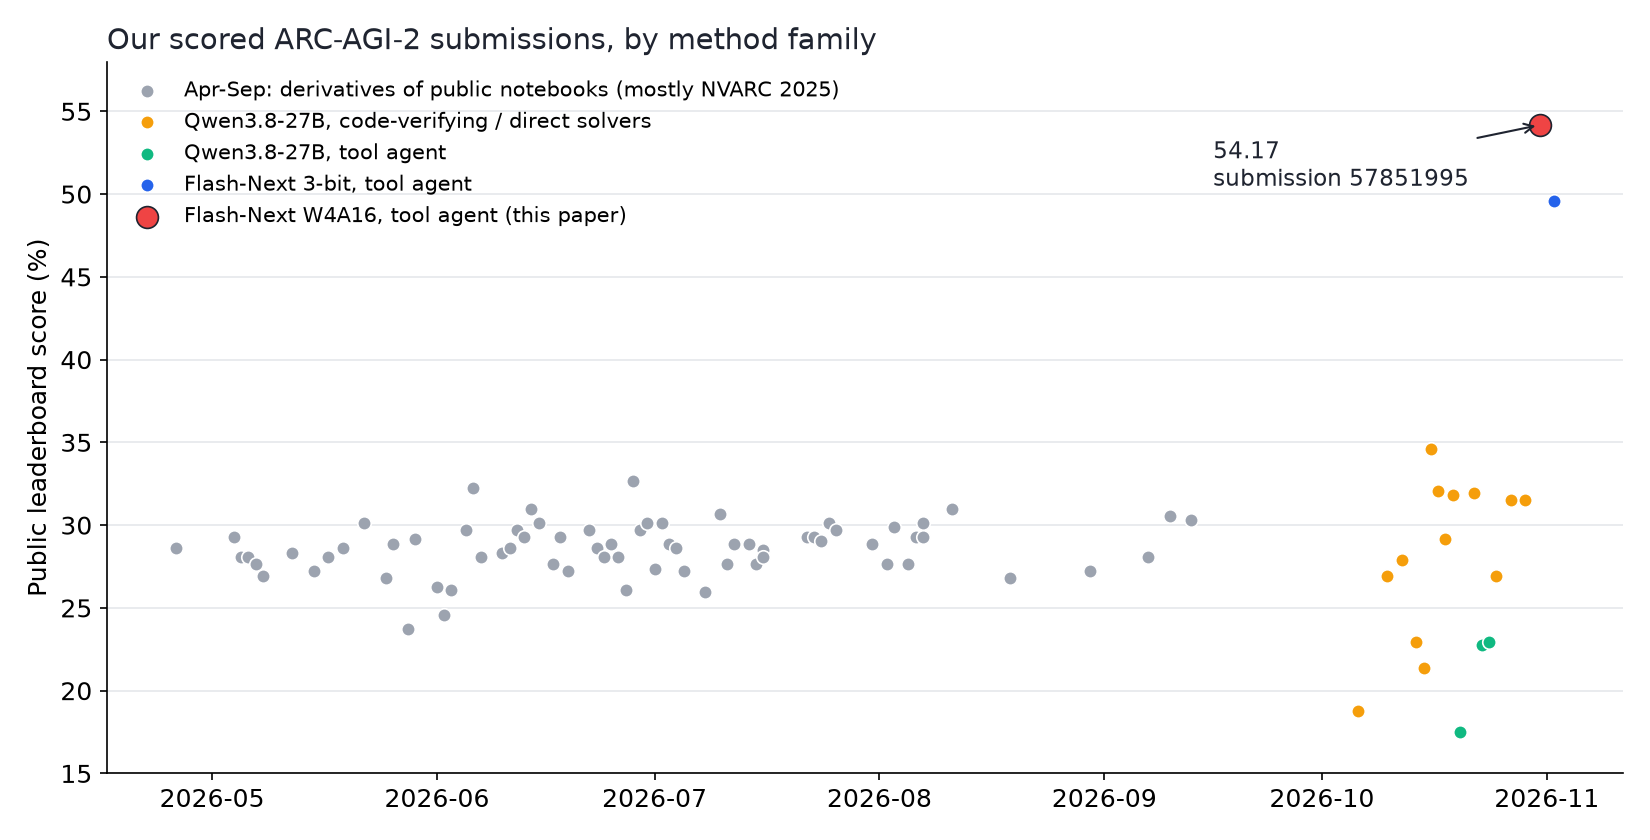
\includegraphics[width=\linewidth]{figures/fig2_lb_history.png}
\caption{Public leaderboard scores of our team's scored submissions (runs that scored below 5 are omitted).}
\label{fig:lb}
\end{figure}

\paragraph{April--September: TTT reproductions.} About 70 submissions built on public NVARC-lineage notebooks scored between 23.75 and 32.64. Paper~1 \cite{paper1} shows why tuning this pipeline gave little: in two logged evaluation runs, 116--117 of 172 test inputs had no correct candidate at all, while better selection could add at most 4.67--7.67 points.

\paragraph{October: Qwen3.8-27B, direct and refine.} A Poetiq-style direct solver on Qwen3.8-27B reached 34.58 with 60k thinking tokens per attempt. The same family at 77.8k tokens scored 21.39 although its evaluation score was 48.61\,\%: on the 240-task hidden run, a longer cap reached fewer tasks. At 49k tokens the score fell to 32.08. Coverage, not per-task skill, set the score.

\paragraph{October: Qwen3.8-27B as a tool agent.} Our first Duck-style agent scored 17.50--22.92. Its first call to the checker came at a median of about 55k tokens: the model solved in its head before using the tool, and attempt budgets of 35--45k tokens left few sessions with a passing program.

\paragraph{November: Qwen3.8-Flash-Next.} Switching to the sparse model with the same agent gave 54.17 (W4A16, this paper) and 49.58 (3-bit ``klee100'' build).

\section{System}
\begin{figure}[t]
\centering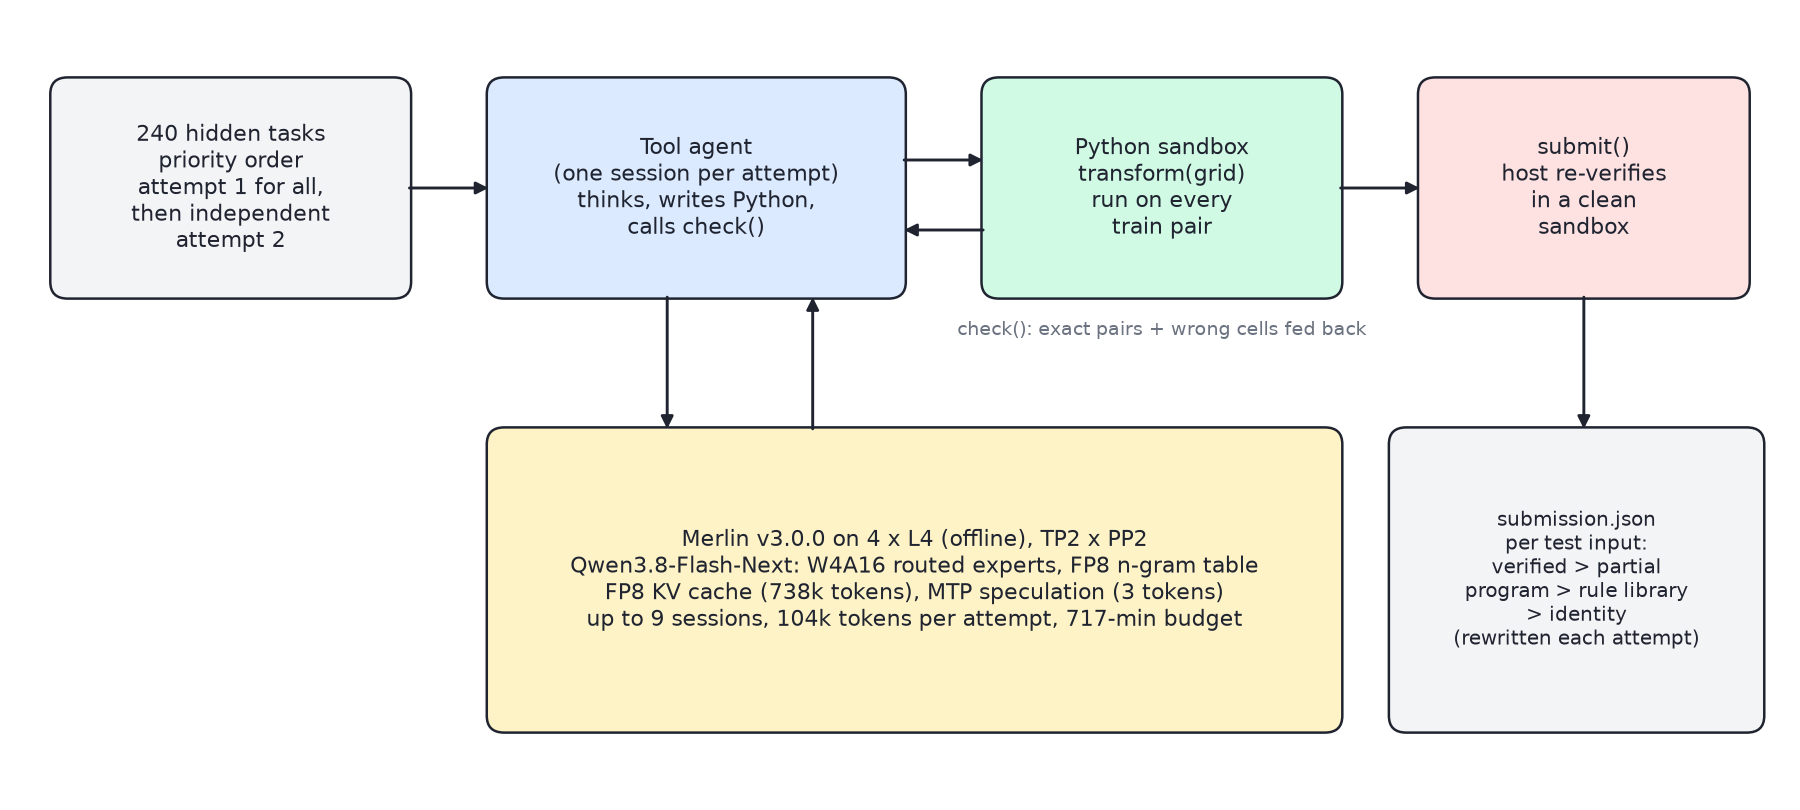
\includegraphics[width=\linewidth]{figures/fig1_pipeline.png}
\caption{Pipeline of submission 57851995.}
\label{fig:pipe}
\end{figure}

\subsection{Model and engine}
Qwen3.8-Flash-Next is a 48-layer mixture-of-experts model with 512 routed experts per layer and top-10 routing, plus a large n-gram embedding table \cite{qwen38}. Table~\ref{tab:hp} lists the serving settings.
\begin{table}[t]
\centering\small
\begin{tabular}{@{}ll@{}}
\toprule
Item & Setting \\
\midrule
Routed experts & W4A16, five checkpoint shards \\
Embedding table (PLE) & FP8 overlay \\
KV cache & FP8 E4M3, static scales; pool 738{,}142 tokens \\
Speculation & MTP, 3 draft tokens, probabilistic acceptance (median accept length 2.88) \\
Concurrency & 9 agent sessions, slot-based admission \\
Engine memory & pinned-memory ladder (3.55\,GB, then 0.75 / 0.5 / 0), QSA prefill-workspace patch, \\
 & shared draft workspace, prefix caching \\
Attempt budget & 104{,}000 tokens per attempt, 2 attempts per task \\
Run budget & 12\,h $-$ 3\,min; failed boot $\to$ next memory step ($\le$3 tries); stalled server relaunched \\
Throughput & 225 tok/s steady median, 172 tok/s window mean (15-task run) \\
\bottomrule
\end{tabular}
\caption{Serving settings of submission 57851995.}
\label{tab:hp}
\end{table}

\subsection{Agent}
Each attempt is one session with a stateful Python sandbox:
\begin{enumerate}
\item The model receives the task and reasons.
\item It writes Python, including a \texttt{transform(grid)} function, and runs it in the sandbox.
\item \texttt{check()} runs \texttt{transform} on every training pair and returns per-pair accuracy and cell differences.
\item The model edits the program until all pairs pass or the budget ends.
\item \texttt{submit()} records the program's output on the test input(s).
\end{enumerate}
Answers are program outputs, so the model never transcribes a 30$\times$30 grid by hand. The sandbox fails closed: a crash or time-out gives no answer instead of a malformed grid.

\subsection{Scheduling and submission}
Attempt~1 runs for every task first, in a fixed priority order; attempt~2 is an independent new session. The two sessions' answers fill \texttt{attempt\_1} and \texttt{attempt\_2}. A complete \texttt{submission.json} with a fallback answer for every test input is written at the start of the run and rewritten at the end, so a crash late in the run cannot void the submission. The commit run executes the same code on three evaluation tasks (3/3 correct, zero errors) before the hidden rerun.

\section{Results}
\subsection{Leaderboard}
\begin{table}[h]
\centering\small
\begin{tabular}{@{}lr@{}}
\toprule
Method family (best submission) & Public LB (\%) \\
\midrule
NVARC-lineage TTT reproductions & 32.64 \\
Qwen3.8-27B, direct / refine (60k tokens) & 34.58 \\
Qwen3.8-27B, tool agent & 22.92 \\
Qwen3.8-Flash-Next 3-bit (klee100), tool agent & 49.58 \\
\textbf{Qwen3.8-Flash-Next W4A16, tool agent (57851995)} & \textbf{54.17} \\
\bottomrule
\end{tabular}
\caption{Best public leaderboard score per family. The public leaderboard uses about half of the 240 hidden tasks.}
\label{tab:lb}
\end{table}

\subsection{Controlled measurements}
\paragraph{FP8 versus BF16 KV cache.} On 15 evaluation tasks chosen as 7 easy, 5 medium and 3 hard, with equal 4{,}050\,s windows, two 104k-token attempts and the same seed, FP8 and BF16 KV each solved 13 tasks (18/20 test outputs; McNemar $p=1.0$, 2 discordant tasks). FP8 doubled the KV pool (214 vs 112 blocks), fitting 9 sessions instead of 5, and raised the steady decode median from 169 to 225 tok/s. The sample is too small to prove parity; it shows no measurable loss.

\paragraph{Precision of the training-pair check.}
\begin{figure}[t]
\centering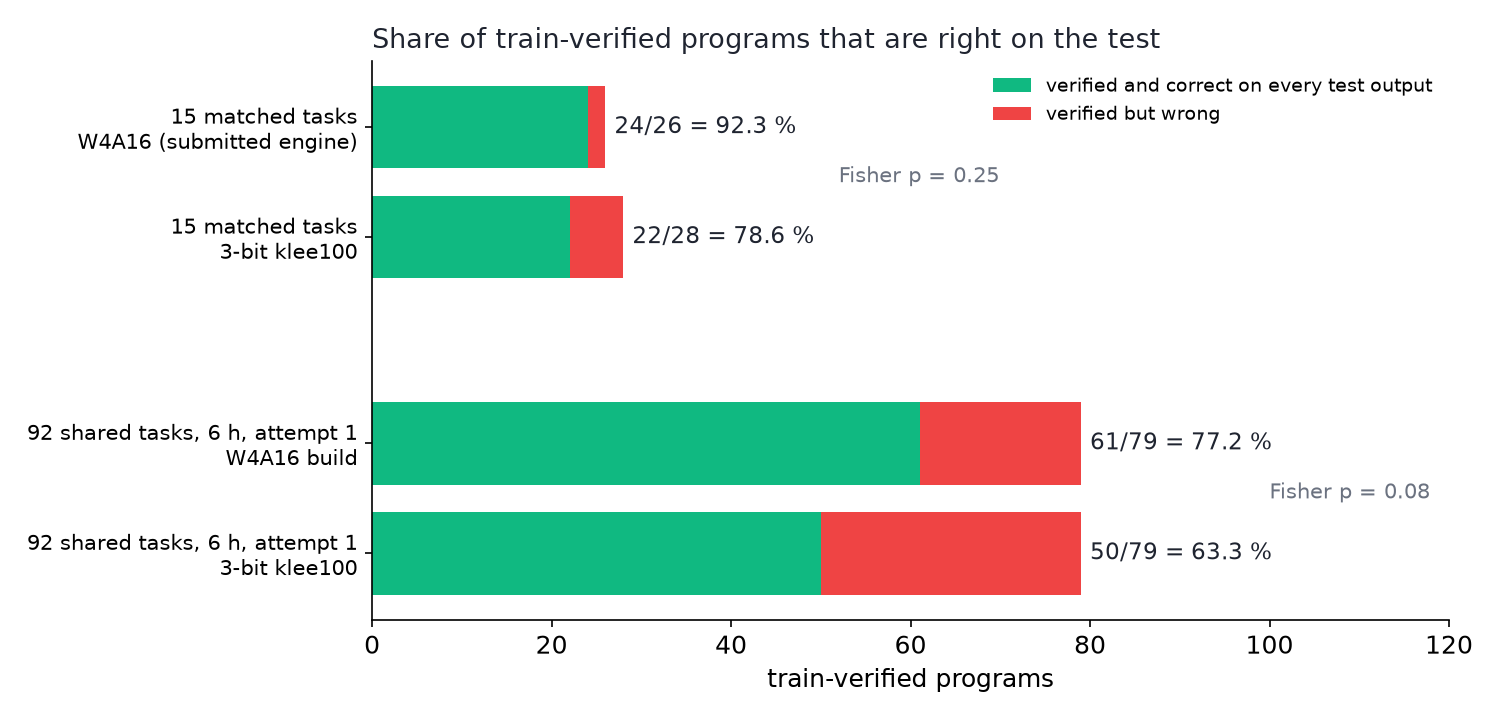
\includegraphics[width=0.85\linewidth]{figures/fig3_verification.png}
\caption{Submitted attempts that passed every training pair, split by correctness on the test output. W4A16: 30 attempts on 15 tasks. 3-bit: 60 attempts on 30 tasks.}
\label{fig:ver}
\end{figure}
Of 30 W4A16 attempts, 26 passed every training pair and were submitted, and 25 of them were correct (Figure~\ref{fig:ver}); the other 4 never passed (3 cut by the time window, 1 by the token budget). The 3-bit build had 54 train-passing submitted attempts out of 60, of which 41 were correct and 13 wrong; on the same 15 tasks it had 8 train-passing wrong answers against W4A16's 1. It also used 1.44$\times$ the tokens of W4A16 on those tasks.

\paragraph{Second attempts.} Over the 90 attempts above, attempt~2 rescued one task in 30. Nearly all solves came from attempt~1.

\paragraph{Coverage in a 6-hour evaluation run.} In a 6-hour run on the 120 public evaluation tasks, a W4A16 build fully solved 63 tasks: 44 of the first 60 in queue order and only 19 of the last 60. The faster 3-bit build solved 74, spread evenly (39 and 35), and answered 107 of 172 test outputs, our best single evaluation run. The 12-hour submission runs the W4A16 build twice as long.

\subsection{Evaluation is a weak proxy for the leaderboard}
The 3-bit build beat W4A16 on evaluation (74 vs 63 tasks in 6 hours) but lost on the leaderboard (49.58 vs 54.17). Our 77.8k-token 27B solver scored 48.61\,\% on evaluation but 21.39 on the leaderboard. We also ran two public Flash-Next notebooks by other teams on the evaluation set under equal 5\,h\,23\,min windows: the one with the higher evaluation score (87.79\,\% of outputs) has the lower published leaderboard score (77--78 vs 83.47). The run lengths, task counts and the public-evaluation tasks' use in training data all differ from the hidden test, so we report evaluation results as mechanism evidence only.

\section{Why it works}
\paragraph{The training pairs are a free unit test.} A short program that reproduces every demonstration very likely encodes the task rule; a typed grid carries no such evidence. With W4A16 Flash-Next, a passed check meant a correct answer 25 times in 26. The 27B agent could not use this filter because it rarely reached a passing program within budget.

\paragraph{Quantization error appears as false verification.} The 3-bit build produced more train-passing programs per hour, but more of them fitted the demonstrations without capturing the rule (13/54 wrong vs 1/26). Throughput benchmarks and teacher-forced divergence do not show this; only end-to-end verified-answer precision does. For a verifying agent, the right objective for quantization and speed choices is correct answers per hour, not tokens per second.

\paragraph{Memory is the binding resource on L4.} Each session holds up to about 100k tokens of context. 4-bit experts make the model fit, and the FP8 KV cache doubles the number of sessions that fit next to it. MTP speculation then raises tokens per second without changing the sampling distribution.

\paragraph{A budget model explains the ranking.} The submitted run has $717$ minutes. At the measured steady rate of 225 tok/s it can generate about 9.7\,M tokens, or about 40k tokens per hidden task; at the 172 tok/s window mean it is about 31k. In the 15-task run, correct first attempts on easy tasks used a median of 6.3k tokens, on medium tasks 32.7k, while hard tasks used 90k and more without success. So the budget covers the easy and medium tasks of the whole queue only if hopeless attempts do not consume it, which is where the queue-order split above shows losses. The same arithmetic explains the 27B history: a 77.8k cap reached fewer hidden tasks than a 60k cap and lost 13 points.

\paragraph{Coverage still limits the score.} The queue-order split of the 6-hour run shows that the late part of the queue is where W4A16 loses tasks. Any gain in speed that keeps verification precision converts directly into score.

\section{What did not work, and a path toward 85\,\%}\label{sec:progress}
\paragraph{Negative results} (from our 27B runs; details in the artifacts):
\begin{itemize}
\item \emph{Early stopping of hopeless thinking.} The best text signal (self-correction churn) separated failing from succeeding attempts with AUC about 0.63, saved only 3--4\,\% of tokens, and out of sample lost 18\,\% of train-passing attempts.
\item \emph{Pause and resume} of long attempts at 30--60k tokens was worse than a straight run at every budget.
\item \emph{Shorter thinking caps} below about 60k tokens (49k) lowered the leaderboard score (32.08 vs 34.58), and longer ones (77.8k) lowered it more (21.39).
\item \emph{Task ordering} by predicted difficulty from the task JSON did not beat a simple priority order, which itself beat random order by 4--7 points under a 50--70\,\% budget.
\item \emph{A dense 27B tool agent} (Section~\ref{sec:journey}) scored below the same model answering directly.
\end{itemize}

\paragraph{Headroom from complementary methods.} On the 120 public evaluation tasks (172 test outputs), the union of all our own runs up to the competition deadline answered 143 outputs (task-normalised 85.69\,\%), although our best single run answered 107. Adding two public Flash-Next notebooks by other teams, run by us under equal windows, the union reaches 162 of 172 (95.56\,\%), and only 10 outputs in 7 tasks were never answered by any system we ran. Different systems fail on different tasks, so the remaining gap is mostly one of selection and budget, not of capability.

\paragraph{Concrete next steps.}
\begin{enumerate}
\item \emph{Speed without false verification}: accept a faster quantization or decoding change only if it keeps train-pass precision (measured as in Figure~\ref{fig:ver}).
\item \emph{Verified-wrong detection}: 1 in 26 (W4A16) to 13 in 54 (3-bit) train-passing answers were wrong; a second check (e.g.\ consistency on augmented copies of the demonstrations) targets exactly these.
\item \emph{Budget routing}: give second attempts only to tasks without a train-passing program, since attempt~2 rescued 1 task in 30.
\item \emph{Portfolio}: run complementary solvers on the tasks the agent leaves unverified, using the union headroom above.
\end{enumerate}

\section{Universality, limitations and threats}
\paragraph{Universality.} The recipe (a sparse model at low precision, a stateful code tool, and a verifier built from the task's own examples) applies wherever candidate solutions can be executed and checked against given examples, for example program synthesis from examples, data-transformation scripts or spreadsheet formulas.
\paragraph{Limitations.}
\begin{itemize}
\item The leaderboard figure is one run on the public half of the hidden set; repeated runs of one of our notebooks varied by about $\pm$1.5 points.
\item Controlled measurements use 15 or 30 tasks and builds that are close to, but not identical with, the submitted one (the 6-hour W4A16 run had extra speed settings).
\item We did not fine-tune any model, and we did not measure the submitted build on all 120 evaluation tasks.
\item Qwen3.8 models may have seen public ARC data in pre-training; we cannot measure this.
\end{itemize}

\section{Conclusion}
A 512-expert reasoning model served at 4 bits with an FP8 cache and speculation on four L4 GPUs, inside an agent that only submits training-checked program output, scored 54.17 on the ARC-AGI-2 public leaderboard, 20 points above our best dense-model and TTT results. The measurements point to one practical rule for fixed hardware: choose quantization, speed and scheduling by verified-answer precision and coverage together.

\section*{Reproducibility and artifacts}
Public notebook: \url{https://www.kaggle.com/code/foysalemonshanto/q27-xhigh-e25-nb6-submit} (version~1, submission~57851995). Its inputs are the Merlin environment, the five W4A16 shards, the FP8 PLE overlay and the agent payload dataset listed in the notebook. Papers and figures: \url{https://www.kaggle.com/datasets/foysalemonshanto/arc2026-hack2publish-papers}.

\section*{Use of AI tools}
AI coding and writing assistants were used to write analysis scripts and draft text. All numbers were taken from saved run outputs and checked by the authors.

\bibliographystyle{plain}
\bibliography{refs}
\end{document}
